%!TEX root = ../Main.tex

\chapter{Introduction}
\label{cha:Introduction}
  \todo[inline]
  {
    General introduction to computer graphics. One of the biggest problems: Performance. Especially with virtual reality.

    Maybe mention the author's (that's me!) bias towards game development
  }

  The field of computer graphics poses many challenges.

  Data is consumed by a pipeline and transformed by complex algorithms, resulting in another set of data that is used in further processing. This transformation process is usually referred to as ``rendering''. In its most simple form, the output of the rendering process is used to present a graphical representation of the input data to the user, typically via a computer monitor peripheral device.

  Computer graphics is an area of computer science that has many disciplines. Examples are \acrfullpl{gui}, computer vision, sprite graphics, and \acrshort{3d} modelling. Most relevant to this paper is \acrfull{3d} computer graphics. \todo{Mention how Vulkan is not only suited for \acrshort{3d} graphics?} The most typical use case in \acrshort{3d} computer graphics is to process data, usually three-dimensional geometric data, in order to produce a 2D image which is then presented to the user with the help of a computer monitor. This processing of data is referred to as \textit{3D rendering} or simply \textit{rendering}.

  While 3D rendering can be implemented in software, special hardware called a \acrfull{gpu} can be used instead to achieve better performance. The need for such hardware already indicates one of the greatest challenges in 3D computer graphics: performance. The amount of data involved in 3D rendering can become quite large. As an example, assume the following:

  \todo{Explain what a Vertex is and how graphics hardware produces faces etc.}

  The aforementioned three-dimensional geometric data can be given in many different ways. The ideal way of representing specific data depends on the use case and the entire 3D graphics pipeline.

  For the sake of illustration, let's assume a data set that consists only of 3D vertices. In this example, each vertex only has a position defining the absolute location of the vertex in 3D space. This position value is stored as a vector of three floating point numbers. Typically, such floating point numbers are standard IEEE floating point numbers (as per IEEE 754), taking up 32 bits or 4 bytes of memory. Thus, each vertex takes up $3*4 = 12$ bytes of memory.

  On desktop systems, applications typically don't access the graphics hardware directly. They instead communicate with a driver that manages hardware access. Communication between an applicatin and the driver is done via an \acrfull{api}. Figure \ref{fig:AppApiDriverOverview} visualizes this relationship. Ideally, the application does not need to know which specific driver it is communicating with as long as the driver is compliant to the \acrshort{api} specification. This abstraction decouples the application from the hardware and enables it to run on systems with different hardware configurations without altering the application itself. It also enables hardware vendors to manipulate or even reject operations requested by the application, typically to enforce some user-specified global settings. \todo{Explain what kind of settings? Maybe give an example?}

  \begin{figure}
    \caption{Interaction between the application and the hardware via the API.}
    \centering
    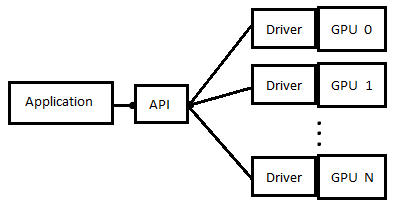
\includegraphics{Main/Images/Application_API_Driver_Overview}
    \label{fig:AppApiDriverOverview}
  \end{figure}

  \todo{Talk about different kinds of graphics \acrshortpl{api} on different systems (D3D, OpenGL on desktop, maybe Metal for OSX, and special \acrshortpl{api} on consoles.)}


  \section{High Level Graphics Workflow}
    \todo[inline]{General overview of the stages several resources (vertices, textures, etc.) have to go through}


  \section{Motivation for a new Graphics API}
    \todo[inline]{Basically write why Vulkan is needed.}

    Graphics hardware is changing rapidly through the years and is highly specialized to do computational work in a massively parallel manner. This makes it not only suitable for graphics computation, but also for general-purpose parallelization of working with large sets of data. These \acrshortpl{api} have grown with the hardware, constantly adapting to it, adding new versions that support different kinds of features and provide different kinds of extensions while maintaining backwards compatability as much as possible. This lead to very complicated \acrshortpl{api} that was getting harder and harder to understand with each new release, especially for beginners.

    But not only graphics and compute hardware has changed. The drivers accompanying the hardware also have to stay backwards compatible. They hide and abstract a lot of the low-level functionality that is needed to work properly with the hardware. This abstraction means that the application developer has less control over what is actually done with the data fed to drivers. Since driver's rarely get information about the exact intent of what the developer plans to do with the supplied data, they have to implement heuristics to decide the best course of action.

    This level of abstraction has been critiqued by many professional developers over the years, demanding for more low-level control. On gaming consoles, low-level control of the hardware was always required (except for Microsoft platforms). This meant that console developers were already used to thinking about data flow on a low level.

    Another aspect is the advent of multi-core CPUs for personal computers in the mid 2000's. Multithreading has become common in CPU programming to achieve better performance. Older graphics \acrshortpl{api}, however, were designed to run on a single thread all the time. Even though these \acrshortpl{api} provide limited support for multithreading by now, they were still originally not designed for it, making it rather difficult to fully utilize multicore performance.

    \todo[inline]{Talk about new \acrshortpl{api} such as D3D12, Mantle, Metal, and also talk about consoles (no specs) that all adress these problems.}


  \section{The Vulkan Graphics and Compute API}
    \todo[inline]{What does it do. Where does it come from. What are people expecting from it. Cross-platform nature (in comparison maybe to PS4's libGNM made specifically for PS4 hardware).}

    \todo[inline]{Insert missing references.}
    The Vulkan \acrfull{api} was designed by the Khronos Group in collaboration with many industry representatives, including Valve Coroporation, AMD, NVIDIA. Version 1.0 of the Vulkan specification was released on the 16th February in 2016. It was designed to provide low-level control to the developer when interacting with graphics and compute hardware.

    Vulkan was designed with a variety of goals in mind.

    \begin{itemize}
      \item Cross-platform
      \item Keep driver complexity at a minimum
      \item Less driver-side CPU overhead
      \item Enable developers a lot of control over the hardware.
      \item Consistent API
    \end{itemize}

    There are many different kinds of hardware configurations today, ranging from high-end gaming systems to mobile platforms such as smartphones. Vulkan is designed to be used with all of these systems. There will be no special version of Vulkan dedicated to embedded systems as was the case with OpenGL ES.

    As a result of striving for less driver overhead, Vulkan also provides the possibility of reducing CPU and GPU power consumption. The driver implementation will have to make fewer guesses of what the host application is trying to do. It is up to the application developer to tell the Vulkan driver exactly what needs to be done. This way the driver only does as much work as it needs to function properly and less power will be consumed. Hardware vendors will also have an easier time providing robust drivers with less bugs due to reduced complexity.

    Another advantage of Vulkan, being a new API built without worrying about backwards compatability, is the chance of designing a new and consistent API so developers will have an easier time creating applications. For more information about the API structure and common patterns in Vulkan, see chapter \ref{cha:VulkanOverview}.

    Version 1.0 of Vulkan was not entirely built in-house at Khronos Group but is in part based on components of AMD's Mantle API, which was donated to the Khronos Group.


    \subsection{Vulkan Competitors}
      \todo[inline]{OpenGL, Direct3D11, Direct3D12, libGNM (PS4), OpenCL}

      Other \acrshortpl{api} exist that are direct competitors to Vulkan.

      OpenGL is Vulkans predecessor and provides a higher level of abstraction from the hardware. It is a very successful API running on several different platforms with varying hardware configurations. Due to it's level of abstraction, OpenGL drivers are very complex and do a significant amount of work on the CPU in order to match abstract commands to the hardware.

      Special flavors of OpengGL exist, such as OpenGL for Embedded Systems, also known as OpenGL ES or GLES, which is a subset of OpenGL to enable hardware-accelerated graphics processing on embedded systems such as smartphones and tablets.

      The Direct3D family of \acrshortpl{api} is developed by Microsoft and only supports Microsoft platforms such as the Windows operating system or the Xbox gaming console. The most recent versions of Direct3D are Direct3D11 and Direct3D12. Direct3D11 provides a higher level of abstraction from the hardware, not unlike OpenGL. It has been around since the release of Windows 7 in 20??\todo{date}. Direct3D12, the latest revision of the Direct3D specification released in 2015\todo{exact date?}, is comparable to Vulkan in the sense of hardware abstraction. It provides much more control to the developer over the hardware.

      \todo[inline]{Mac OS X: Metal}

      \todo[inline]{Gaming console graphics libraries.}

      \todo[inline]{OpenCL as compute API}


  \section{Document Structure}
    \todo[inline]{The structure and content of this document.}

    \lipsum
